%\documentclass[preprint]{aastex}
\documentclass[twolcolumn,apj]{emulateapj}
\usepackage{ctable}
\usepackage{amsmath}
\usepackage{graphicx}
%\usepackage[figuresright]{rotating}
%\usepackage{rotating}
%\usepackage{natbib}
%\usepackage{pdflscape}
%\usepackage{lscape}
%\citestyle{aa}

\def\b{\mathbf{b}}
\def\k{\mathbf{k}}
\def\r{\mathbf{r}}
\def\q{\mathbf{q}}
\def\b{\mathbf{b}}
\def\kp{\mathbf{k}^\prime}
\def\kpp{\mathbf{k}^{\prime\prime}}
\def\V{\mathbb{V}}
\def\At{\tilde{A}}
\def\Vt{\tilde{V}}
\def\Tt{\tilde{T}}
\def\tb{\langle T_b\rangle}
\newcommand{\vis}{\mathbf{v}}
\newcommand{\x}{\mathbf{x}}
\newcommand{\xhat}{\hat{\mathbf{x}}}
\newcommand{\A}{\mathbf{A}}
\newcommand{\y}{\mathbf{y}}
\newcommand{\N}{\mathbf{N}}
\newcommand{\Nfg}{\mathbf{N}_{\textrm{fg}}}
\newcommand{\Q}{\mathbf{Q}}
\newcommand{\M}{\mathbf{M}}
\newcommand{\W}{\mathbf{W}}
\newcommand{\G}{\mathbf{G}}
\newcommand{\Rfg}{\mathbf{R}_{\textrm{fg}}}
\newcommand{\rhat}{\hat{\mathbf{r}}}
\newcommand{\Nbl}{N_{\textrm{bl}}}

\newcommand{\acl}[1]{{\color{red} \textbf{[ACL:  #1]}}}
\definecolor{applegreen}{rgb}{0.55, 0.71, 0.0}
\newcommand{\mep}[1]{{\color{applegreen} \textbf{[MEP:  #1]}}}

\renewcommand{\topfraction}{0.85}
\renewcommand{\bottomfraction}{0.1}

\begin{document}

%\title{What Power Spectrum Measurements From the Next Generation of 21~cm Experiments Can Teach Us About the Epoch of Reionization}
\title{Global signal interferometer (XXX: replace with better title)}

\author{Morgan E. Presley\altaffilmark{1},
}
\altaffiltext{1}{Department of Astrophysical Sciences, Princeton University, Princeton NJ}

\begin{abstract}
Really great abstract
\acl{Hey, look at these fun commands.}
\mep{Here's yours.}
\mep {Check out all the colors!!! http://latexcolor.com/}
\end{abstract}


\keywords{reionization, dark ages, first stars --- techniques: interferometric}

\section{Introduction}
\begin{itemize}
\item Say why 21cm is important.
\item Narrow focus to global signal.
\item Survey of current instruments and efforts.
\item Challenge of foregrounds.
\item Why an interferometer might be helpful plus why we're not crazy (Ekers + Rots Theorem?).  Angular info helps with foreground suppression.
\item Preview results (exquisite extraction; great foreground mitigation; high significance detection).
\item ``The rest of this paper is organized as follows..."
\end{itemize}

\section{Why we're really not crazy}
\begin{itemize}
\item Cartoon / qualitative picture?
\item Simple eqn. showing that there is non-zero response?
\item Intuitive, qualitative description of what sort of arrays are good.  (Preview for later sections).
\item Discussion of noise bias and other problems with single dipole experiments?
\end{itemize}

\section{Mathematical formalism}
\begin{itemize}
\item How does one actually get from visibilities to a global signal measurement.
\item The error statistics that come for free.
\item Quantification of leakage from other spherical harmonics.
\end{itemize}

In order to obtain a global signal measurement from visibilities, it is necessary to invert the linear equation 
\begin{equation}
\y = \Q \mathbf{x} + \mathbf{n}
\end{equation}
where $\y$ is a vector of length $\Nbl$ containing the visibilities measured at different baselines, $\mathbf{n}$ is the contribution of noise from both foregrounds and systematics, and $\mathbf{x}$ is a projection of the true sky onto the spherical harmonics $Y_{\ell m}(\theta,\phi)$. As such, $\mathbf{x}$ has length $(\ell_{\textrm{max}}+1)^2$, where $\ell_{\textrm{max}}$ is the largest $\ell$ value used in the model of the true sky. The matrix $\Q$ is the beam response of an antenna array at different baselines (rows) and different spherical harmonics (columns). $\Q$ is determined by 
\begin{equation}
\textrm{Q}_{j,\ell m} = \int d \boldsymbol \theta^2 A(\boldsymbol \theta) Y_{\ell m}(\boldsymbol \theta) e^{2\pi i \frac{\mathbf{b_\textit{j}}}{\lambda} \cdot \boldsymbol \theta}
\end{equation}
where $\boldsymbol \theta$ is the angular position on the sky, $A$ is the primary beam for the antennas, $\mathbf{b_{\textit{j}}}$ is the $j$th baseline, and $\lambda$ is the wavelength of observation. Since $\Q$ is not in general invertible, we cannot solve for $\mathbf{x}$ directly and instead can only recover an estimator for $\mathbf{x}$. We can define a general estimator of the form 
\begin{equation}
\mathbf{\hat x} = \M \Q^\dagger \N^{-1} \y
\end{equation}
where $\N$ is the total noise covariance matrix and M is some matrix chosen by the data analyst. One useful choice for $\M$ is 
\begin{equation}
\M = [\Q^\dagger \N^{-1} \Q]^{-1}
\label{eqn:M}
\end{equation}
which is obtained through a least-squares derivation that minimizes $\chi^2 \equiv (\y-\Q \mathbf{\hat x})^\dagger \N^{-1} (\y-\Q \mathbf{\hat x})$. Note that for this choice of $\M$, the ensemble average of $\mathbf{\hat x}$ is $\mathbf{x}$.
Using this fact, we can directly find the covariance of $\mathbf{\hat x}$ to be 
\begin{equation}
\textrm{Cov}(\mathbf{\hat x}) = [\Q^\dagger \N^{-1} \Q]^{-1}
\label{eqn:Covxhat}
\end{equation}
as shown in \citet{Tegmark_CMB_maps_wli}. \mep{Is this properly cited?}. Therefore, using equation (\ref{eqn:M}) for our statistical analysis allows us to analytically find the error statistics if the noise covariance matrix for the foregrounds and systematics is known. However, since galactic foreground models are not well constrained, it is not safe to assume we know $\N_{\textrm{fg}}$. Consequently, Monte Carlo simulations are still necessary to determine the error bars on measurements analyzed using this method. Note, however, that although we do not know the exact noise covariance $\N$, there is nothing wrong with choosing equation (\ref{eqn:M}) for our data analysis, as long as we do not claim that our error bars are constrained by equation (\ref{eqn:Covxhat}). %-- it just may not be optimal.

Note that two inverses must be taken in order to compute $\M$. In general, neither $\N$ nor $\Q^\dagger \N^{-1} \Q$ will be invertible, requiring us to approximate both inverses with a pseudo-inverse. We used a pseudo-inverse method that raises the value of the small eigenmodes, inverts, and then projects out those small eigenmodes, as laid out in the appendix of \citet{Tegmark_CMB_spectra_wli}. \mep{Is this how I should cite this?} \mep{Is there something significant I need to say about this method, or is it pretty standard?}

Since $\Q$ is not diagonal, higher spherical harmonic modes will leak into our measurement $\y$. If it were possible to do the inverses in equation \ref{eqn:M}, then these leakages could be dampened down by taking the ensemble average of many observations. This is because 
\begin{equation}
<\xhat> = \M \Q^\dagger \N^{-1} \Q \x
\end{equation}
which is equal to $\x$ if $\M$ is the true inverse of $\Q^\dagger \N^{-1} \Q$. In order to quantify the relative amount of leakage from the different modes, it is convenient to define a window function matrix $\W$ as 
\begin{equation}
\W = \M \Q^\dagger \N^{-1} \Q. 
\end{equation}
With this definition, the elements of the first row of the window function matrix quantifies the ratios between the contributions from the different modes. A good experimental design would result in a very high ratio between $W_{0,00}$ and all of the other $W_{0,\ell m}$.

\mep{Figure time! Show the green/pink plots of 1st row of window function for different arrays.}

\begin{figure}[h]
	\centering
	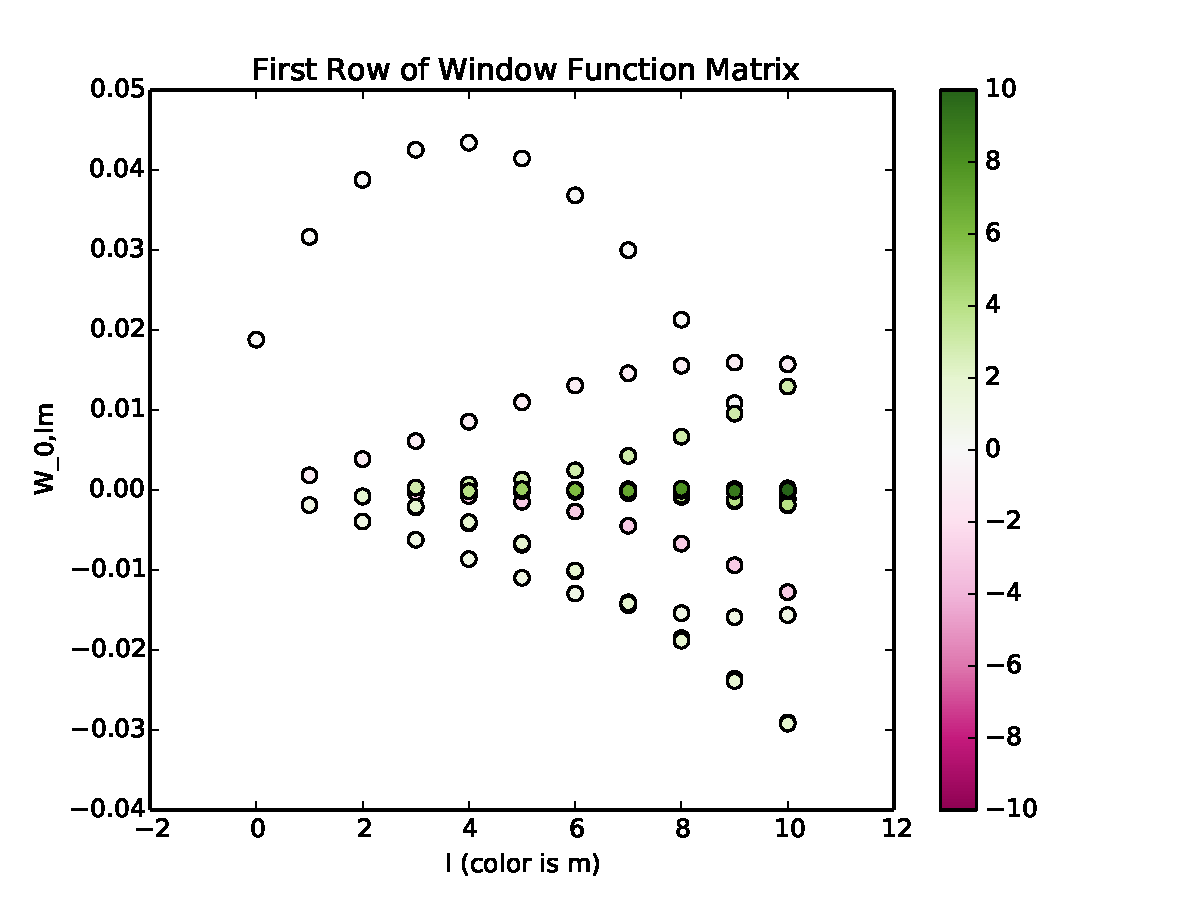
\includegraphics[width=3in]{figures/W_matrix_filler.pdf}
	\caption{\mep{Of course, this will have to be updated when the new data comes in. Probably to show several figures for different arrays?}\mep{Uh.... Weird stuff happens if I try to make the figure bigger. It's not wrapping the text and is trying to keep the figure in the column somehow?? Not sure what's up with the formatting style here.}}
	\label{fig:WindowFunction}
\end{figure}

\acl{The tone of the writing is excellent, btw.}

\section{Exploration of arrays}
\begin{itemize}
\item Show plots of different arrays that we tried.
\item (Maybe spherical harmonic plots with fringe patterns overlaid on spherical harmonics).
\item Reasoning behind our crazier-looking arrays.
\item Rules of thumb for designing a global signal interferometer.
\end{itemize}

\section{Foregrounds and their mitigation}
\begin{itemize}
\item General characteristics of foregrounds.
\item Desire to avoid using too much spectral information because the signal itself is a spectrum.
\item How to use angular information.
\item (Modifications to array design to account for foregrounds).
\end{itemize}

The primary source of contamination in a global signal experiment comes from galactic foregrounds, which make extraction of the global signal difficult for a number of reasons. Primarily, the galactic foregrounds are many orders of magnitude brighter than our expected signal, so finding the global signal through a simple spatial average over the sky would result in a measurement dominated by foregrounds. Also, since both the galactic foregrounds and the expected global re-ionization signal are spectrally smooth, foreground subtraction techniques will likely be unreliable. Therefore, we propose using angular information to differentiate galactic foregrounds from the global signal. 

Our ultimate goal in foreground analysis is to construct a noise covariance matrix for the foregrounds: $\Nfg$. $\Nfg$  shows the correlation between the Fourier modes probed by the antenna array, and hence has dimensions $\Nbl \times \Nbl$. One method \mep{Are there other methods?} to generate $\Nfg$ from a model of the sky is to first find a covariance matrix of the sky $\Rfg$ and transform that matrix into the Fourier domain of the visibilities via the matrix transformation 
\begin{equation}
\Nfg = \mathbf{G} \Rfg \mathbf{G}^\dagger
\end{equation}
Since $\Rfg$ has dimensions $N_{\textrm{pix}} \times N_{\textrm{pix}}$, note that $\mathbf{G}$ must have dimensions $\Nbl \times N_{\textrm{pix}}$. Although $\mathbf{G}$ serves a purpose similar to a Fourier transformation matrix, it is not precisely a Fourier matrix as that would probe every single possible Fourier mode, and we only want those that correspond to our array's baselines. As such, $\mathbf{G}$ is defined by 
\begin{equation}
G_{i,j} = A(\rhat_j)e^{2\pi i \frac{\mathbf{b_\textit{i}}}{\lambda} \cdot \boldsymbol \rhat_j} \Delta \Omega
\end{equation}
where $\rhat_j$ is the angular position of the $j$th pixel,  $\Delta \Omega$ is the solid angle encompassed by each pixel, and $\mathbf{b_\textit{i}}$ is the $i$th baseline. 

\mep{Insert here stuff on how you're calculating $\Rfg$?}

\acl{An interesting point I just realized.  We can make the argument that since the normalization of $\mathbf{N}$ scales out of the expression for $\hat{\mathbf{x}}$, our foreground mitigation scheme is a very conservative one that only uses shape information, and not the detailed spectral form of our foreground model.}
\acl{Somewhere, we also need to address rotation synthesis}
\acl{Also need to add noise to simulations}.

\section{Monte carlo / foreground simulation results}
\begin{itemize}
\item $\mathbf{N}_\textrm{fg}$ might not be properly modeled, so we can't use $[\mathbf{Q}^\dagger \mathbf{N}^{-1} \mathbf{Q}]^{-1}$ as a reliable indicator of the errors.  (Although recall that it's a perfectly fine choice for extracting the signal).
\item To get reliable estimates...Monte Carlo!
\item Really great results! (Error bars and covariance on the recovered spectra).
\end{itemize}

\section{Fisher matrix results}
\begin{itemize}
\item Fisher matrix formalism for translating error statistics from recovered spectra to parameterizations of the signal.
\end{itemize}

\section{Conclusions}
\begin{itemize}
\item This is a great way to do this measurement.  It will produce lots of great science! And eternal glory!
\end{itemize}

\bibliographystyle{apj}
\bibliography{globalSig}{}

\end{document}
